Como mencionamos antes, en este capítulo se presentaran las modificaciones que se implementaron sobre los algoritmos que se describieron anteriormente. Éstos cambios apuntan a mejorar la calidad de las soluciones, haciendo hincapié en los valores \texttt{inter} de los paquetes pero al mismo tiempo sin descuidar los buenos resultados que se habían obtenido.

Además de las mejoras descriptas, mostraremos nuevos procedimientos basados en búsquedas tabú, que demostraron ser muy útiles y eficientes en todos los casos. También se incluye una alternativa completamente diferente a los algoritmos del estilo \texttt{Produce\allowbreak-and\allowbreak-Choose} influenciado por las soluciones del estilo \emph{greedy}.

\section{Produce-and-Choose}
En general los algoritmos de la clase \texttt{Produce\allowbreak-and\allowbreak-Choose} genera una cierta cantidad de paquetes y luego se seleccionan los que pertenecerán a la solución.

Los parámetros del algoritmo son los del problema mencionado en~\autoref{introduccion:problemaFormal}: el conjunto de ítems $I$, el atributo complementario $\alpha$, la función de presupuesto $f: 2^{I} \rightarrow \rm I \!R$, el limite del presupuesto $\beta$, un valor $0 < \gamma < 1\ \in \rm I \!R$ para ponderar si se quiere paquetes más cohesivos o no y una cantidad $k$ de paquetes a generar. El algoritmo devuelve un conjunto de paquetes válidos.

\begin{center}
	\begin{algorithm}[H]
	\DontPrintSemicolon
	\SetAlgoLined
		\KwData{$I,\alpha,f,\beta,k,\gamma$}
		\KwResult{Conjunto válido de $k$ paquetes}
		$cand \leftarrow ProduceBundle(I,\alpha,f,\beta)$\;
		$G \leftarrow BuildBundleGraph(cand)$\;
		\Return $ChooseBundles(k,\gamma,G)$\;
	\caption{Produce-and-Choose}\label{alg:PAC}
	\end{algorithm}
\end{center}

La función \texttt{ProduceBundle} genera un conjunto de paquetes candidatos, en las siguientes secciones se presentarán y analizarán las diferentes estrategias que fueron usadas y se detallara su funcionamiento.

\texttt{BuildBundleGraph} recibe el conjunto de paquetes candidatos y devuelve un grafo completo con peso en las aristas y en los vértices. Cada vértice representa un paquete del conjunto de candidatos y el peso del vértice es el valor \texttt{intra}, mientras que el peso de las aristas representa el valor \texttt{inter} entre los paquetes correspondientes a cada nodo. 

Finalmente la función \texttt{ChooseBundles} busca el \textit{subgrafo-k} que maximice el peso de los vértices y aristas. En este punto también se analizarán distintas implementaciones. Finalmente los vértices del \textit{subgrafo-k} corresponderán a los paquetes pertenecientes a la solución.

Como se puede observar la estructura de esta familia de algoritmos permite la facilidad de introducir mejoras en las dos fases críticas: generación y selección de paquetes. Permitiendo al mismo tiempo combinar cada una de ellas de la mejora manera dependiendo del objetivo de la búsqueda requerida.

\subsection{Mejoras en la generación de paquetes}
La generación de paquetes se puede realizar a través de un proceso de agrupación de un conjunto de objetos que son parecidos. Este proceso conocido como ``agrupamiento'' consiste en juntar objetos basándose en la información que estos describen o en sus relaciones. El objetivo es que los objetos del grupo sean similares entre sí y diferentes de los objetos de los restantes grupos. Cuanto mayor la similitud dentro del conjunto (valor \texttt{intra}) y mayor sea la diferencia entre conjuntos el agrupamiento será mejor.

La noción de que es un grupo correctamente constituido no puede ser definido con presición y es por tal motivo que existe una gran cantiad de algoritmos de agrupamiento \cite{Estivill-Castro:2002:WSM:568574.568575}. Sin embargo, se puede definir ambiguamente como un conjunto de objetos relacionados entre sí. Dependiendo del modelo de repsentación usado para el problema, dependerá el tipo de algoritmo que será utilizado.

Por ejemplo, para los veinte puntos de~\autoref{res:img-howToCluster} existen tres (o más) formas de agruparlos que son válidas y que dependen del contexto. Si es por que los puntos estén juntos, entonces la estructura más razonable es en la que existen dos grupos. Pero la división de los dos grupos en tres subgrupos es más intuitiva para el ojo humano. Tampoco es irracional decir que los puntos pertenecen a cuatro conjuntos. Por lo tanto la mejor definición de cómo se debe realizar la agrupación depende del contexto de los objetos que se quieren agrupar y del problema.

\begin{figure}[H]
  \centering
   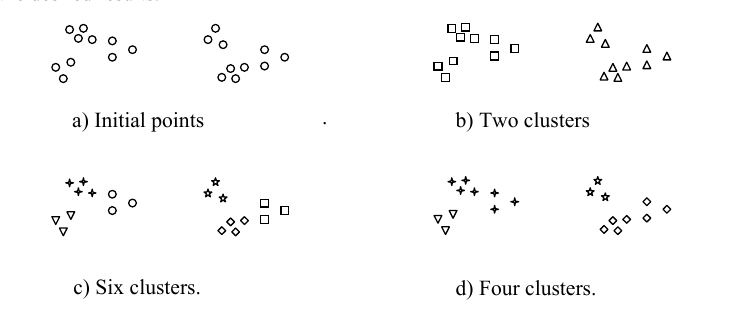
\includegraphics[width=0.8\textwidth]{img/howToCluster.png}
   \caption{}
   \label{res:img-howToCluster}
\end{figure}
En este trabajo el agrupamiento esta definido para que cada grupo contenga la máxima cantidad de items sin exceder el presupuesto. La agrupación se realiza por la similitud de los objetos, que se obtiene a través de la función de similitud, para que los items dentro del grupo sean lo más parecidos posible y así obtener paquetes cohesivos.

En la literatura se pueden encontrar diferentes tipos de algoritmos de agrupamiento, la gran mayoría pueden categorizarse entre los particionales y los jerárquicos \cite{opac-b1087461}. Los métodos particionales seleccionan un número definido de $k$ centroides iniciales, $k$ será el número final de grupos finales. Cada objeto será asignado al paquete que le sea más cercano y luego iterativamente los elementos serán reubicados de un grupo a otro. Éste tipo de métodos requieren que la cantidad de grupos a generar sea preestablecida. 

A diferencia de los métodos particionales, los jerárquicos construyen grupos mediante la partición recursiva de los grupos de objetos y no requieren predefinir una cantidad de grupos a generar. A su vez éstas técnicas se suelen subdividir en dos estrategias: algomerativas y divisivas, las cuales serán detalladas más adelante.

En esta tesis se plantearon dos mejoras para el algoritmo jerárquico \textit{Constrained hierarchical agglomerative clustering} presentado en el artículo \cite{journals/tkde/Amer-YahiaBCFMZ14}: (1) La función que se utiliza para decidir qué \textit{clusters} se unen. (2) La complejidad algorítmica. En las próximas secciones se describen detalladamente los pasos elegidos.

En relación al algoritmo \textit{BOBO}, también descripto en la publicación mencionada en el párrafo anterior, se mantuvo sin cambios en pos de realizar comparaciones entre los resultados obtenidos a través de las mejoras propuestas y las obtenidas mediante la implementación original.

\subsubsection{Bundles One-By-One}
El método \texttt{BOBO-k}, que está inspirado en k-means, consiste en generar $k$ paquetes del conjunto de $n$ ítems. El algoritmo comienza con todos los items del conjunto $I$ como posibles pivots $P$. Se selecciona un pivote de $P$ y con los elementos de $I$ se genera un paquete válido ``alrededor'' de este, en caso que el paquete generado sea suficientemente bueno se agrega al conjunto de candidatos y los ítems del paquete se eliminan de $I$. La generación de paquetes continúa hasta que se cumpla el criterio de parada, generar $k$ paquetes válidos.

\begin{center}
	\begin{algorithm}[H]
	\DontPrintSemicolon
	\SetAlgoLined
		\KwData{$I,\alpha,f,\beta,\mu,\text{ cantidad de paquetes }c$}
		\KwResult{Conjunto válido de paquetes}
		$pivots \leftarrow I$\;
		$cand \leftarrow \emptyset$\;
		\While{$ \left|C\right| < c\ and\ P \neq \emptyset$}{
			$pivot \leftarrow SelectPivot(pivots)$\;
			$bundle \leftarrow BuildBundle(pivot,I,\alpha,f,\beta)$\;
			\eIf{$Score(bundle) \geq \mu$}{
				$cand \leftarrow cand \cup \left\{bundle\right\}$\;
				$I \leftarrow I \setminus \left\{bundle\right\}$\;
				$pivots \leftarrow pivots \setminus \left\{pivot\right\}$\;
			}
			{
				$pivots \leftarrow pivots \setminus \left\{pivot\right\}$\;
			}
		}
		\Return $cand$\;
	\caption{BOBO-k}\label{alg:bobo}
	\end{algorithm}
\end{center}

La función \texttt{selPivote} selecciona un pivote perteneciente al conjunto de pivotes, en este trabajo se siguió con la recomendación de \cite{Zhang:2002:ESI:638644.638646} de que la selección sea aleatoria. La función \texttt{BuildBundle} genera un paquete a partir del pivote. Se trata de una función que implementa un algoritmo goloso dado que que en cada iteración se agrega al paquete que se genera el ítem del conjunto $I$ que maximiza la función intra y que cumple con las restricciones de la complementariedad y el presupuesto. La función \texttt{Score} calcula el valor intra del paquete. Se dice que un paquete es suficientemente bueno si el valor intra supera el umbral establecido por $\mu$.

\subsubsection{Constrained hierarchical agglomerative clustering}
Anteriomente se indicó que el agrupamiento jerárquico suele clasificarse en algoritmos \textit{aglomerativo} y \textit{divisivo}. El aglomerativo, comienza con cada objeto perteneciente a su un grupo unitario y en cada iteración se intentará unir dos grupos generando un nuevo y de esa manera se logra subir de jerarquía, el algoritmo es conocido como \textit{hierarchical agglomerative clustering} (HAC) \cite{journals/tkde/Amer-YahiaBCFMZ14}. La estrategia divisiva, en cambio, comineza con todos los objetos en un mismo grupo y en cada paso se realizan divisiones, generando que un grupo descienda en la jerarquía hasta no lograr más subdivisiones.

Comúnmente a los algoritmos algomerativos (HAC desde ahora en adelante) se los puede visualizar como un dendograma, como se ve en la~\autoref{nuevaspropuestas:dendograma1}. En el eje X se encuentran los objetos que van a ser agrupados y en la coordenada Y se haya la distancia en la que los elementos se unirán. Las uniones de los objetos se representan mediante una línea vertical que comienza a la altura de la distancia en la que los grupos han sido unidos. Por ejemplo, en la figura mencionada, el grupo \textit{4} se une al \textit{5} en la distancia 2 formando el \textit{cluster B}. En un paso posterior éste último se unirá al grupo \textit{3} en una distancia cercana a 3 obteniendo el nuevo \textit{cluster C}. En cada paso se generará una nueva unión hasta que solo quede un solo grupo.

\begin{figure}[H]
  \centering
    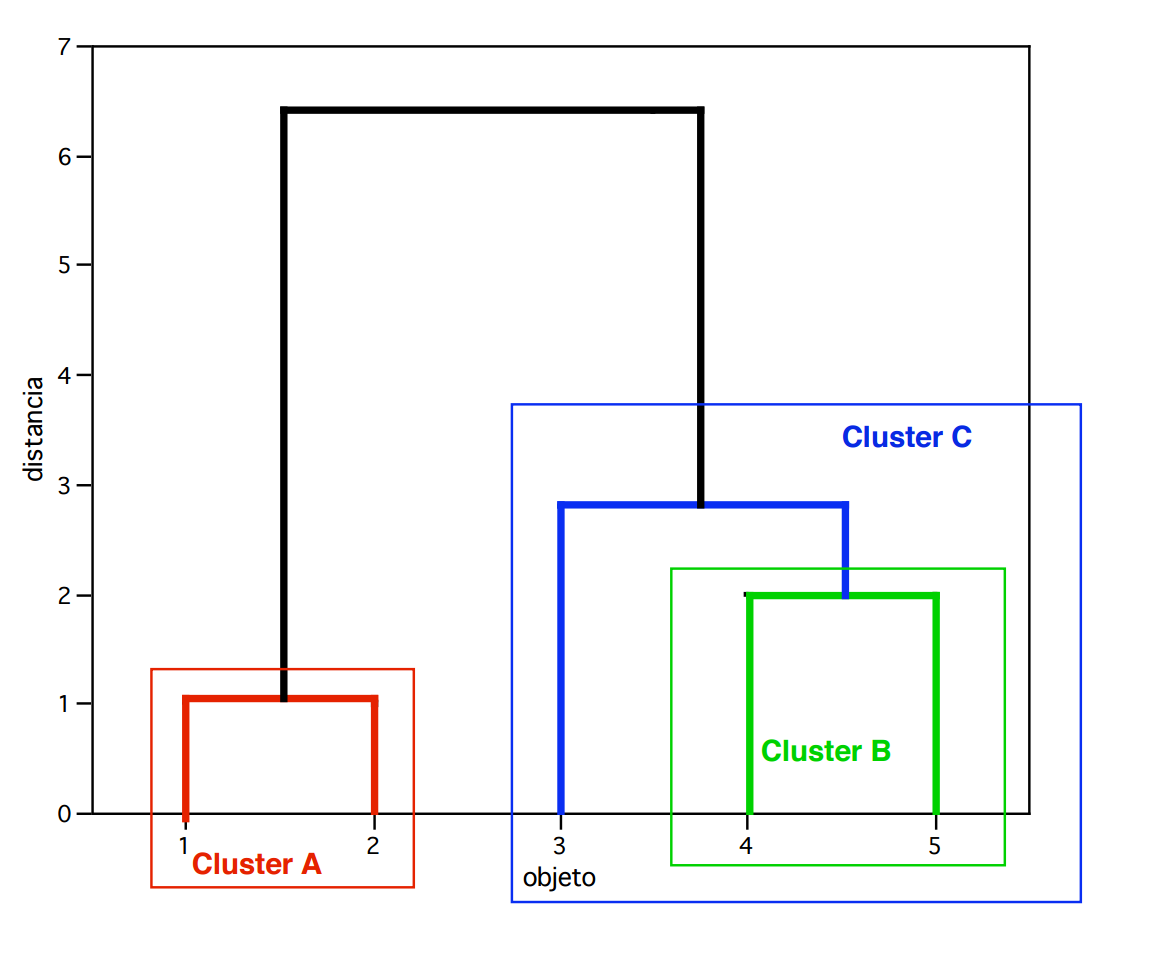
\includegraphics[width=0.5\textwidth]{img/dendograma01.png}
  \caption{Dendrograma}
  \label{nuevaspropuestas:dendograma1}
\end{figure}

Cortando el dendograma mediante líneas horizontales se puede determinar el número de paquetes o \emph{clusters} en el que se dividirá el conjunto de objetos inicial. En la~\autoref{nuevaspropuestas:dendograma2} parte a) se puede ver que aplicando un corte en la distancia 5 se obtienen 2 paquetes, en cambio si se aplicara a una distancia mayor a 2 se obtendrían 3 paquetes como se puede observarse en la parte b) de la misma figura.

\begin{figure}[H]
  \centering
    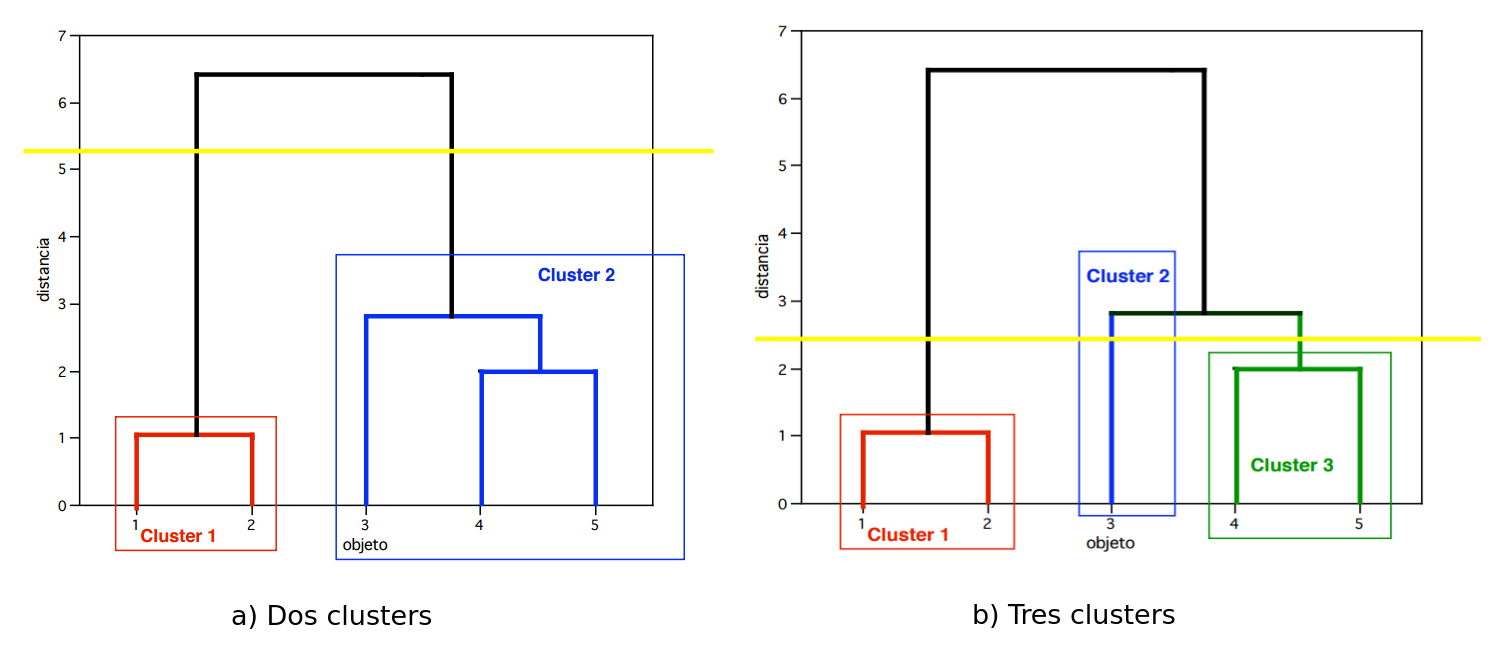
\includegraphics[width=1\textwidth]{img/dendograma02.png}
  \caption{Cortes en el dendrograma}
  \label{nuevaspropuestas:dendograma2}
\end{figure}

El algormitmo llamado \textit{Constrained hierarchical agglomerative clustering} (C-HAC), más adelante se detallara, es una modificación aplicada sobre la técnica HAC descripta en los párrafos anteriores. La idea prinicipal es agregar restricciones pertenecientes al problema puntual que presentamos en este trabajo. Por ejemplo, supongamos que se quiere realizar la unión de los grupos $S_1$ y $S_2$. Si el grupo resultante $S_1 \cup S_2$ es inválido, o sea, no cumple con las reglas de complementaridad o de presupuesto definadas al cominezo del problema, entonces el algoritmo no aplicará dicho agrupamiento.

\begin{center}
	\begin{algorithm}[H]
	\DontPrintSemicolon
	\SetAlgoLined
		\KwData{$I,\alpha,f,\beta,\gamma,\text{ cantidad de paquetes }c$}
		\KwResult{Conjunto válido de paquetes}
		$cand \leftarrow \bigcup_{i \in I}\left\{i\right\}$\; \label{alg:C-HAC:init}
		\While{$ \left|cand\right| > c$}{ \label{alg:C-HAC:cycleOutter}
			$bestScore \leftarrow -\infty$\;
			$bestCandidate \leftarrow \emptyset$\;
			\ForEach{$S_i\in cand$}{ \label{alg:C-HAC:cycleInner}
				\ForEach{$S_j\in cand; S_i \neq S_j$}{ \label{alg:C-HAC:cycleInnerInner}
					\If{$ValidMerge(S_i,S_j,\alpha,f,\beta)$}{ \label{alg:C-HAC:validMerge}
						\If{$Score(S_i \cup S_j) \geq bestcore$}{ \label{alg:C-HAC:score}
							$bestScore \leftarrow score(S_i \cup  S_j)$\;
							$bestCandidate \leftarrow \left\{S_i,S_j\right\}$\;
						}
					}
				}
			}
			\If{$bestCandidate = \emptyset$}{
				$break$\;
			}
			$cand \leftarrow cand \setminus \left\{S\right\}$ $(\forall S \in bestCandidate)$\;
			$cand \leftarrow cand \cup bestCandidate$\;
		}
		\Return $cand$\;
	\caption{C-HAC}\label{alg:C-HAC}
	\end{algorithm}
\end{center}

A continuación explicaremos en detalle el\textbf{~\autoref{alg:C-HAC}}. Como puede observarse, se ejecuta $N - c$ (\textit{~\autoref{alg:C-HAC:cycleOutter}}) veces, donde $N$ es la cantidad de items. En cada paso de la iteración principal se unirán los dos grupos de elementos con mayor similitud y que a su vez sea una unión válida. Cada uno de los ciclos interiores (\textit{~\autoref{alg:C-HAC:cycleInner} y~\autoref{alg:C-HAC:cycleInnerInner}}) itera sobre los elementos contenidos en el conjunto grupos candidatos a unir, realizando comparaciones entre todos los grupos que existentes hasta el momento. Tomando como peor caso que cada iteración tenga $N$ pasos, el orden de complejidad de \texttt{C-HAC} es $\mathcal{O}(N^{3})$. La función \textit{Score} que se utiliza para decidir qué {\em clusters} unir sólo toma en cuenta el valor \texttt{intra}, por lo que dicha operación puede ser tratada como constante ya que se trata de número fijo de comparaciones.

La propuesta de esta tesis es incluir el valor \texttt{inter} de los paquetes en la selección del par de {\em clusters} en pos de lograr un mejor criterio de unión como consecuencia obtener soluciones de mayor calidad. Por este motivo se definió la función \textit{Intra-Inter} en reemplazo de la función \textit{Score}. Entonces, para \textit{Intra-Inter} dados dos {\em clusters} $C_i$ y $C_j$ sean

$$A(C_i,C_j) = \sum_{u \in C_i, v \in C_j}{s(u,v)},$$

$$E(C_i,C_j)=\max_{u \in C_i, v \in C_j}{s(u,v)} \qquad \mbox{ y}$$

$$\mbox{Intra-Inter}(C_i,C_j) = \gamma A(C_i,C_j) + t (1-\gamma) E(C_i,C_j)$$

De esta manera el {\em cluster} resultante incrementará el valor intra y se habrán unido dos {\em clusters} con alta similitud favoreciendo la dispersión en el {\em clustering} final. El factor $t$ intenta equilibrar los dos términos de esta sumatoria, ya que de lo contrario el segundo resultará siempre despreciable con respecto al primero. En este trabajo el valor que se le asigna a $t$ corresponde a la cantidad de similitudes que se suman en A, o sea $\frac{(\#C_i + \#C_j) \cdot (\#C_i + \#C_j - 1)}{2}$  

Si bien el objetivo principal de la modificación propuesta es aumentar la calidad de las soluciones, también se tuvo en cuenta un aspecto fundamental como es la complejidad temporal del algoritmo. De lo contrario el uso de las mejoras propuestas no hubieran podido ser usadas en las pruebas que en los próximos capítulos detallaremos, por tratarse de instancias con miles de objetos.

Recapitulando las fórmulas presentadas anteriormente, para evitar realizar el cálculo desde cero de $A$ y $E$ para todo par de {\em clusters} en todas las iteraciones de la etapa \emph{Produce} del algoritmo, se  mantienen estructuras con esos valores, cuya actualización se realiza en tiempo constante a partir de las siguientes relaciones entre la iteración $r$ y $r-1$:

$$A^r(C_i \cup C_j, C_s) = A^{r-1}(C_i,C_s) + A^{r-1}(C_j,C_s) \quad \mbox{ y}$$

$$E^r(C_i \cup C_j,C_s) = \max (E^{r-1}(C_i,C_s),E^{r-1}(C_j,C_s))$$

El valor de la función Intra-Inter para cada {\em cluster} es almacenado en orden decreciente en una cola de prioridad. La implementación de colas de prioridad permite el borrado e inserción en $O(\log n)$, resultando la complejidad total del algoritmo $O(n^2 log n)$.

Para mejorar la complejidad del algoritmo de \texttt{C-HAC} e incluir la información inter-paquete, aquí se propone el algoritmo \texttt{Intra-Inter C-HAC}, el cual tiene una complejidad $\mathcal{O}(N^{2}\lg n)$. La similitud entre los grupos se guarda en colas de prioridad en orden decreciente, entonces la cola $P\left[k\right].max()$ devuelve el grupo de mayor similitud con el k-ésimo grupo. Luego de combinar los grupos $\omega_{k_{1}}$ y $\omega_{k_{2}}$, $\omega_{k_{1}}$ se utiliza como la representación. Para $\omega_{k_{1}}$ se calcula la similitud con el resto de los grupos y se actualiza en las colas de similitud. Para identificar entre dos grupos que la unión es inválida por alguna de las restricciones, en las colas de similitud el valor de la similitud es $-1$.

\begin{center}
	\begin{algorithm}[H]
	\DontPrintSemicolon
	\SetAlgoLined
		\KwData{$I,\alpha,f,\beta,\gamma$}
		\KwResult{Conjunto válido de paquetes}
		\ForEach{$S_i\in I$}{
			\ForEach{$S_j\in I$}{
				\eIf{$validMerge(S_i,S_j,\alpha,f,\beta)$}{
					$C[i][j].sim \leftarrow Score(S_i \cup S_j)$\;
				}
				{
					$C[i][j].sim \leftarrow -1$\;
				}
				$C[i][j].index \leftarrow j$\;
			}
			$I[i] \leftarrow 1$\;
			$P[i] \leftarrow $ priority queue for $C[i]$ sorted on sim\;
			$P[i].Delete(C[i][i])$ \tcc*[f]{se elimina así mismo de la pila}\;
		}
		$A \leftarrow []$\;
		\For{$k \leftarrow 1$ to $I.length$}{
			$k_1 \leftarrow \max_{k:I[k]=1}{P[k].max().sim}$\;
			\If{$validMerge(S_i,S_j,\alpha,f,\beta)$}{
				$break$\;
			}
			$k_2 \leftarrow P[k_1].max().index$\;
			$A.Append(\left\langle k_1,k_2 \right\rangle)$\;
			$I[k_2] \leftarrow 0$\;
			$P[k_1] \leftarrow []$\;
			\For{$i$ with $I[i]-1 \vee i \neq k_1$}{
				$P[i].Delete(C[i][K_1])$\;
				$P[i].Delete(C[i][k_2])$\;
				\eIf{$validMerge(S_i,S_j,\alpha,f,\beta)$}{
					$C[i][k_1].sim \leftarrow Inter-Intra(i,k_1 \cup k_2,\gamma)$\;
					$C[k_1][i].sim \leftarrow Inter-Intra(i,k_1 \cup k_2,\gamma)$\;
				}
				{
					$C[i][k_1].sim \leftarrow -1$\;
					$C[k_1][i].sim \leftarrow -1$\;
				}
				$C[i][k_1].index \leftarrow i$\;
				$C[k_1][i].index \leftarrow i$\;
				$P[i].Insert(C[i][k_1])$\;
				$P[K_1].Insert(C[k_1][i])$\;
			}
		}
		\Return $A$\;
	\caption{Intra-Inter C-HAC}\label{alg:Intra-Inter C-HAC}
	\end{algorithm}
\end{center}

\subsection{Modificaciones en la selección de paquetes}
El segundo paso de los algortimos del estilo \emph{Produce and Choose} luego de la producción de paquetes es la selección de los $k$ mejores que formarán parte de la solución final. A continuación se detallará el comportamiento de la implementación orignal de \cite{journals/tkde/Amer-YahiaBCFMZ14} y los cambios propuestos.

El problema puede representarse como un de grafo completo con pesos en las aristas y vértices. Los nodos corresponden a los paquetes generados en la primer parte del algoritmo y su peso equivale a su calidad o valor \texttt{intra}. Las aristas representan la distancia existente entre los nodos y su peso está corresponde con el valor \texttt{inter} de los paquetes involucrados. Teniendo en cuenta la transformación mencionada recientemente se puede interpretar que la solución de encontrar aquellos paquetes que maximicen la función objetivo es equivalente a encontrar un k-subgrafo completo de mayor peso.

La definición formal de encontrar el subgrafo completo de tamaño k de peso máximo entre nodos y vértices es la siguiente: dado el grafo $ G = (V,E) $, la funciones de peso $\psi : E \rightarrow \Re$ y $\omega : V \rightarrow \Re$, el entero $ k \leq |V| $ y el real $\gamma \in [0,1]$. La salida es el conjunto $V' \subseteq V$ tal que $|V'| = k$ y que maximiza el peso de los nodos y vértices del subgrafo $G' = (V', E')$ ponderado por el parámetro $\gamma$.

\begin{equation}
\gamma \sum_{v \in V'}{\omega(v)} + (1 - \gamma) \sum_{(u,v) \in E'}{\psi(u,v)}
\end{equation}

El problema previamente mencionado puede reducirce a la ya conocida situación de hallar el k-subgrafo más denso \cite{DBLP:journals/algorithmica/FeigePK01}. Transformando el grafo del problema original a un grafo ponderado, en el que el peso de los vértices esta dado por la siguiente función:
 
\begin{equation}
\omega(u,v) = \dfrac{\gamma}{2( k - 1)} (\omega(u) + \omega(v)) + (1 - \gamma)\psi(u,v) 
\end{equation}

En \cite{journals/tkde/Amer-YahiaBCFMZ14} proponen utilizar la heurística \ref{alg:chooseBundles} para hallar el k-subgrafo de mayor peso de un grafo ponderado. El algoritmo consiste en cada iteración remover un vértice al par con menor peso del grafo hasta que quedarse con un grafo de $k$ nodos.

\begin{center}
	\begin{algorithm}[H]
	\DontPrintSemicolon
	\SetAlgoLined
		\KwData{$k,\gamma,\text{ el grafo con peso en los vértices y aristas }G=(V,E) \text{ donde }\forall S \in V / \omega(S) = \sum_{u,v \in S}{s(u,v)}$ y $\forall (S_i,S_j) \in E / \psi(S_i,S_j) = 1 - \max_{u \in S_i, v \in s_j}{s(u,v)}$}
		\KwResult{Conjunto de k bundles}
		$\omega(u,v) = \dfrac{\gamma}{2( k - 1)} (\omega(u) + \omega(v)) + (1 - \gamma)\psi(u,v)$\;
		$S \leftarrow V$\;
		\While{$ \left|S\right| > k$}{
			$u \leftarrow \min_{u \in S}{\sum_{v \in S}{\omega(u,v)}}$\;
			$S \leftarrow S \setminus  \left\{u\right\} $\;
		}
		\Return $C$\;
	\caption{Selección de paquetes}\label{alg:chooseBundles}
	\end{algorithm}
\end{center}


La debilidad de este algoritmo es que no esta definida la selección, en la arista de menor peso, del nodo a remover. Entonces se puede dar el caso de que el nodo que se remueve es el que pertenece a una solución de mejor calidad.

Por ejemplo si se considera que en la etapa de producción se generan los tres paquetes $A$, $B$ y $C$. En el cual los valores \texttt{Intra} de los paquetes son: $\omega(A) = 5$, $\omega(B) = 5$ y $\omega(C) = 5$. En cuanto a los valor \texttt{Inter} entre los paquetes:$\psi(A,B) = 0$, $\psi(A,C) = 1$ y $\psi(B,C) = 0$. En este escenario para la solución que contenga 2 paquetes y con $\gamma=0,1$ se tiene los siguientes valores para cada par de paquete:
\begin{itemize}
	\item $\omega(A,B) = 0,45$
	\item $\omega(A,C) = 1,15$
	\item $\omega(B,C) = 0,2$
\end{itemize}
 
Siendo el par de paquetes $B, C$ el de menor valor en la función $\omega$, entonces sí el paquete que se remueve es $C$ la solución resultante contiene los paquetes $A$ y $B$. El valor la función objetivo de esta solución generada es $0.9$, mientras que el valor de la función objetivo de la solución que contiene los paquetes $A$ y $C$ es $1,4$.

En este trabajo se propone un nuevo enfoque para seleccionar los paquetes de la solución. En esta propuesta, a diferencia del algoritmo anterior, la solución se genera iterativamente agregando en cada paso el paquete que maximiza la función objetivo hasta alcanzar la cantidad de paquetes requeridos en la solución.

Para los paquetes generados en el ejemplo anterior, en esta propuesta se tiene que para la primer iteración las soluciones posibles son $S^{1}_{1}=\{A\}$, $S^{1}_{2}=\{B\}$ y $S^{1}_{3}=\{B\}$. Siendo que $S^{1}_{1}$ es la solución con mayor valor de función objetivo, en la segunda iteración las posibles soluciones son:  $S^{2}_{1}=\{A,B\}$, $S^{2}_{2}=\{A,C\}$. Quedándose finalmente con la solución $S^{2}_{2}$ que, como se vio anteriormente, es la solución con mayor función objetivo.

En los casos que acá interesa estudiar, en la relación entre la parte \texttt{intra} y la \texttt{inter} de función objetivo es que el valor de la parte \texttt{intra} es considerablemente mayor que el \texttt{inter}. Esto se debe a que en un paquete el valor \texttt{intra} esta dado por la suma de todas las similitudes entre los elementos del paquete, mientras que el valor de la parte \texttt{inter} es de solo una de las relaciones. Además entre una solución $S'$ que contiene $n$ paquetes y la solución $S''$ que contiene $n+1$ paquetes entonces la segunda solución tiene $n$ relaciones inter-paquete más que la primer solución. A continuación se propone una función para este nuevo algoritmo en el que se compensa estas diferencias.

Para el algoritmo \ref{alg:algSelProp} que se propone en esta tesis para la etapa de selección, la función que se utiliza en cada iteración para seleccionar un paquete para la solución es una variante de la función objetivo. En esta función cada parte de la función objetivo es multiplicada por un coeficiente. Con el coeficiente se equilibra la parte \texttt{intra} y la \texttt{inter} durante todo la generación de la solución.   

Formalmente esta función se define como, sea $R$ el conjunto de paquetes producidos y $S \subseteq R$ el conjunto de paquetes seleccionados en la iteración $i$ se agrega a la solución el paquete que cumple con:

\begin{equation}
\max_{b \in (R/S)}{\dfrac{k}{|S|}} \gamma \sum_{v \in \left\{b\right\} \cup S}{\omega(v)} + \dfrac{k * (k-1)}{|S| * (|S|-1)} (1-\gamma) \sum_{v,w \in \left\{b\right\} \cup S}{\psi(v,w)}
\end{equation}

\begin{center}
	\begin{algorithm}[H]
	\DontPrintSemicolon
	\SetAlgoLined
		\KwData{$k,\gamma, \text{el grafo con peso en los vértices y aristas } G=(V,E) \text{ donde } \forall S \in V / \omega(S) = \sum_{u,v \in S}{s(u,v)} y \forall (S_i,S_j) \in E / \psi(S_i,S_j) = 1 - \max_{u \in S_i, v \in s_j}{s(u,v)}$}
		\KwResult{Conjunto de k bundles}
		$\omega(u,v) = \dfrac{\gamma}{2( k - 1)} (\omega(u) + \omega(v)) + (1 - \gamma)\psi(u,v)$\;
		$S \leftarrow \emptyset$\;
		$R \leftarrow V$\;
		\While{$ \left|S\right| < k$}{
			$c \leftarrow \max_{b \in (R/S)}{\dfrac{k}{|S|}} \gamma \sum_{v \in \left\{b\right\} \cup S}{\omega(v)} + \dfrac{k * (k-1)}{|S| * (|S|-1)} (1-\gamma) \sum_{v,w \in \left\{b\right\} \cup S}{\psi(v,w)}$\;
			$S \leftarrow S \cup \left\{c\right\}$\;
			$R \leftarrow R \setminus \left\{c\right\}$\;
		}
		\Return $S$\;
	\caption{Selección de paquetes proporcional}\label{alg:algSelProp}
	\end{algorithm}
\end{center}

\section{Algoritmo goloso}

En esta tesis se plantea una alternativa para encontrar una solución al problema de \texttt{Recuperación de Ítems Empaquetados}, en el que se ataquen principalmente dos puntos: (1)que la solución se construya de forma tal que se considere de la misma manera las dos partes de la función objetivo -la parte \texttt{inter} y la \texttt{intra}- y (2)que sea aceptable el tiempo de ejecución para grandes cantidades de ítems. El primero de estos puntos es para tener una variante de \texttt{Produce-and-choose} en el cual por la forma de generar la soluciones se enfocan más en la parte \texttt{intra}, porque primero produce paquetes sin considerar la parte \texttt{inter} de la función objetivo.

Un algoritmo goloso es un tipo de heurística que construye la solución iterativamente seleccionando en cada paso la opción óptima local, esperando así lograr una solución óptima. En la mayoría de los problemas el algoritmo goloso no encuentra la solución óptima, pero son muy usados por su sencillez y velocidad de la ejecución.

Por los motivos mencionados anteriormente y por las características del algoritmo goloso, es que de decidió implementar esta heurística para encontrar una solución. El algoritmo goloso que se propone comienza con con los $k$ paquetes de la solución vacíos y en cada iteración se agrega un ítem, que no pertenece a la solución, en el paquete que maximiza la función objetivo y sin violar las restricciones del problema. El algoritmo finaliza cuando por alguna restricción no es posible agregar más objetos a la solución. Sea $I$ el conjunto de ítems del problema, $\omega$ la función objetivo y en el inicio la solución $S_0 = \emptyset$ y $t=1$ entonces se define $S_t = S_{t-1} \cup \{i\}$ dónde $i \in I$, $i \notin S_{t-1}$ y $S_t$ es una solución válida. 

Como se puede ver, esta implementación prioriza la cantidad de elementos de la solución ante el valor objetivo de la misma. Con esto se quiere decir que en cada paso, si es posible, se agrega un ítem a la solución pese a que disminuya el valor de la función objetivo. Ya que un escenario posible es que $\omega(S_{t-1}) > \omega(S_t)$.

\begin{center}
	\begin{algorithm}[H]
	\DontPrintSemicolon
	\SetAlgoLined
		\KwData{$I,\alpha,f,\beta,k,\gamma$}
		\KwResult{Conjunto válido de paquetes}
		$\omega(S) = \sum_{b \in S}{\sum_{u,v \in b}{\gamma s(u,v)}} + \sum_{b_1,b_2 \in S}{(1-\gamma) (1-\max_{u \in b_1, v \in b_2}{s(u,v)})}$\;
		$cand \leftarrow \bigcup_{1 \ldots k}\emptyset$\;
		$isComplete \leftarrow False$\;
		\While{$isComplete = False$}{
			$bestScore \leftarrow -\infty$\;
			$bestCandidate \leftarrow \varnothing$\;
			$bestBundle \leftarrow \varnothing$\;
			\ForEach{$elem \in I$}{
				\ForEach{$bundle \in cand$}{
					\If{$validMerge(bundle,\{elem\},\alpha,f,\beta)$}{
						$score \leftarrow \omega((Cand \setminus \left\{bundle\right\}) \cup \left\{bundle \cup \left\{elem\right\}\right\})$\;
						\If{$score > bestScore$}{
							$bestScore \leftarrow score$\;
							$bestBundle \leftarrow bundle$\;
							$bestCandidate \leftarrow elem$\;
						}
					}
				}
			}
			\eIf{$bestCandidate \neq \varnothing$}{
				$cand \leftarrow (cand \setminus \left\{bestBundle\right\}) \cup \left\{bundle \cup \left\{bestCandidate\right\}\right\}$\;
				$I \leftarrow I \setminus \left\{bestCandidate\right\}$\;
			}{
				$isComplete \leftarrow True$\;
			}
		}
		\Return $cand$\;
	\caption{Algoritmo heurística golosa}\label{alg:algHeuGol}
	\end{algorithm}
\end{center}

\section{Búsquedas Tabú}
Las búsquedas locales consisten en moverse de solución en solución, aplicando cambios a la solución candidata hasta encontrar una mejor solución o satisfacer un criterio de parada. Los algoritmos comienzan a partir de una solución válida y en cada iteración se mueven a una solución vecina, esto es posible sólo si se puede definir una relación de vecindad en el espacio de soluciones. Como una solución puede tener muchas soluciones vecinas se elige siempre la que maximice (o minimice, según el problema elegido) el criterio seleccionado, esto produce que el algoritmo pueda estancarse en un máximo (ó mínimo) local y nunca pueda salir de él.

\textbf{Tabú search} es una metaheurística para resolver problemas de optimización, de la familia de las búsquedas locales, diseñada para escapar de óptimos locales. Para explorar regiones del espacio de búsqueda que serían dejadas de lado por el procedimiento de búsqueda local, la búsqueda tabú modifica la estructura de vecinos para cada solución a medida que la búsqueda progresa y permite moverse a una solución vecina de menor calidad. De esta manera se permite al algoritmo escapar de máximos (o mínimos) locales.

Las implementaciones de búsqueda tabú utilizan estructuras de memoria, conocidas como listas tabú, que determinan cuáles son las soluciones vecinas permitidas de una solución. Para evitar que soluciones de buena calidad no sean visitadas porque la lista tabú lo prohíbe, se introduce el concepto de criterios de aspiración que permite, bajo ciertas circunstancias, visitar una solución que se encuentra en la lista tabú.

Para alcanzar mejores soluciones se introduce el concepto de criterios de aspiración. Estos determinan cuándo se pueden reemplazar las restricciones tabú, eliminando así la clasificación tabú aplicada a un movimiento. 

Una de las ventajas que tienen este tipo de metaheurísticas es que no son muy costosas en tiempo de ejecución siempre que la cantidad máxima de iteraciones no sea excesiva, con lo cual se puede ejecutar sin problemas y sin importar de que algoritmo de generación y selección provenga la solución original con el fin de intentar mejorarla.

Se implementaron las búsquedas tabú Inter-Paquete e Intra-Paquete. La primera busca encontrar una mejor solución entre la actual y los paquetes ya generados; la otra consiste en mejorar los paquetes con los ítems que quedaron fuera de la solución.

\subsection{Inter-Paquete}
La búsqueda se concibió especialmente para la fase de selección del algoritmo \texttt{Produce and Choose}, es decir en la fase que se selecciona un subconjunto de paquetes de los generados en la fase anterior de producción. De la solución obtenida en la fase de selección se va a realizar la búsqueda tabú con los paquetes generados en la fase de producción con el objetivo de visitar soluciones vecinas y esperando obtener una mejor selección.

Para esta implementación se define que las soluciones vecinas de la solución $S$, son aquellas soluciones que no contienen el paquete con menor valor Inter de $S$ e incluye un paquete que no pertenece a $S$. El paquete que se saca de $S$ se agrega a la lista tabú durante una cantidad establecida de
iteraciones. Esta lista contiene los paquetes que no pueden ser parte de la solución a visitar. Además se define para el criterio de aspiración, admitir una solución vecina que contiene un paquete que esta en la lista tabú si mejora la función objetivo con respecto a la mejor solución encontrada hasta el momento. 

El esquema del proceso para construir una nueva soluci\'on es el siguiente:

\begin{enumerate}
\item $S^* = S$, $ \bar{S}= S$, $LT = \emptyset$

\item Mientras no se cumpla criterio de parada hacer:

\begin{enumerate}
      	
\item Se identifica el paquete $b_r$ en $\bar{S}$ con menor inter:

$$b_r = \argmin_{\scriptscriptstyle b_i \in \bar{S}} \sum_{\substack{\scriptscriptstyle  b_j \in \bar{S} \\ \scriptscriptstyle  b_j \ne b_i}} (1-\max_{\substack{\scriptscriptstyle  u\in b_i \\ \scriptscriptstyle v \in b_j}} s(u,v))$$

\item Se determina el paquete, $b_c$, con menor inter en $\bar{S} \setminus \{b_r\}$
	
\item Se determina el conjunto de paquetes candidatos $C$ como los paquetes de $B\setminus \bar{S}$ que maximizan su inter respecto a $b_c$:

$$C = \argmax_{\scriptscriptstyle b_i \in B \setminus \bar{S}} (1-\max_{\substack{\scriptscriptstyle u\in b_i \\ \scriptscriptstyle v \in b_c}} s(u,v))$$

\item Se determina el mejor paquete de $C$ no prohibido en la lista tabú $LT$ según el criterio:

$$b = \argmax_{\scriptscriptstyle b_s \in C \setminus LT} \sum_{\scriptscriptstyle b_i, b_j \in \bar{S}\setminus \{b_r\} \cup \{b_s\}}(1-\max_{\substack{\scriptscriptstyle u\in b_i \\ \scriptscriptstyle v \in b_j}} s(u,v))$$

\item Se evalúa el criterio de aspiración para los paquetes en $C \cap LT$

$$b_{tabu} = \argmax_{\scriptscriptstyle b_s \in C \cap LT} w(\bar{S} \setminus \{b_r\} \cup \{b_s\})$$

\item Si $\max(w(S^*),w(\bar{S} \setminus \{b_r\} \cup \{b\})) < \qquad \qquad$ $\qquad \qquad w(\bar{S} \setminus \{b_r\} \cup \{b_{tabu}\})$ entonces

$$\bar{S} = \bar{S} \setminus \{b_r\} \cup \{b_{tabu}\}$$ 

Si no $$\bar{S} = \bar{S} \setminus \{b_r\} \cup \{b\}$$

\item Actualizar $LT$

\item Si $w(\bar{S})>w(S^*)$ entonces $S^*=\bar{S}$

\end{enumerate}

\item Retornar $S^*$

\end{enumerate}

\begin{center}
	\begin{algorithm}[H]
	\DontPrintSemicolon
	\SetAlgoLined
		\KwData{$S, cand, \gamma, MAX\_ITER, ITER\_TABU$}
		\KwResult{Conjunto válido de paquetes}
		$\omega(S) = \sum_{b \in S}{\sum_{u,v \in b}{\gamma s(u,v)}} + \sum_{b_1,b_2 \in S}{(1-\gamma) (1-\max_{u \in b_1, v \in b_2}{s(u,v)})}$\;
		$UpdateTabu(S) = \left\{ \left\langle b, n-1 \right\rangle  / \left\langle b, n \right\rangle \in S \wedge n-1 > 0 \right\}$\;
		$Inter(b_1, S) = \sum_{b_2 \in S, b_1\neq b_2}{(1-\max_{u \in b_1, v \in b_2}{s(u,v)})}$\;
		$Inter(S) = \sum_{b_1, b_2 \in S}{(1-\max_{u \in b_1, v \in b_2}{s(u,v)})}$\;
		$iteration \leftarrow 0$\;
		$tabuBundles \leftarrow \emptyset$\;
		$bestSolution \leftarrow S$\;
		$visitSolution \leftarrow S$\;
		\While{$iteration < MAX\_ITER$}{
			$worstBundle \leftarrow \min_{b \in visitSolution \setminus tabuBundles}{Inter(b, visitSolution)}$\;
			$centroidBundle \leftarrow getCentroid(visitSolution)$\;
			$visitSolution_a \leftarrow \max_{b \in cand}{(visitSolution \setminus \left\{worstBundle\right\}) \cup \left\{b\right\}}$\;
			$visitSolution \leftarrow \max_{b \in cand \setminus tabuBundles}{(visitSolution \setminus \left\{worstBundle\right\}) \cup \left\{b\right\}}$\;
			\If{$\omega(visitSolution) > \omega(bestSolution)$}{
				$bestSolution \leftarrow visitSolution$\;
			}
			\If{$\omega(visitSolution_a) > \omega(bestSolution)$}{
				$bestSolution \leftarrow visitSolution_a$\;
				$visitSolution \leftarrow visitSolution_a$\;
			}
			$tabuBundles \leftarrow tabuBundles \cup \left\{\left\langle worstBundle, ITER\_TABU \right\rangle\right\}$\;
			$tabuBundles \leftarrow UpdateTabu(tabuBundles)$\;
			$iteration \leftarrow iteration + 1$\;
		}
		\Return $bestSolution$\;
	\caption{Búsqueda tabú sobre paquetes}\label{alg:algBusTabuBundle}
	\end{algorithm}
\end{center}

\subsection{Intra-Paquete}
El objetivo de la búsqueda Intra-Paquete es buscar una mejor solución a través de generar soluciones con paquetes más cohesivos. En esta búsqueda los vecinos de la solución $S$ son las soluciones a las cuales se le modifica un paquete con alguna de las siguientes acciones que generan un paquete válido: agregar un elemento, quitar un elemento o intercambiar un elemento del paquete con otro elemento que no pertenece a la solución. Para esta implementación existen tres listas tabú: una lista de elementos, una de movimientos y una de paquetes. Los elementos que se encuentran en la lista tabú, no pueden ser seleccionados para incluirse en una solución. Los paquetes de la lista, son los que no pueden ser seleccionados para modificar su estructura para una nueva solución y la lista de movimientos contiene el par de elementos que se intercambiaron para ir de la solución $S$ a $S'$ para que esos elementos no se vuelvan a intercambiar.

La lista de los movimientos se utiliza para evitar ciclar entre las soluciones, por ejemplo si las soluciones visitadas son $S, S_1, \ldots, S_n, S$ prohibiendo que se vuelvan a intercambiar el mismo par de elementos, se asegura que la próxima no sea $S_1$.

El criterio de aspiración que se utiliza es permitir utilizar un elemento de la lista tabú para intercambiar con un elemento de la solución actual, si el valor de la función objetivo es mayor del de la mejor solución encontrada hasta al momento.

De la solución actual se realiza el movimiento a una nueva solución con los pasos:
\begin{enumerate}
	\item Obtener el paquete, $p$, menos cohesivos de la solución $S$.
	\item Crear el paquete $p'$ válido agregando un elemento que no pertenezca a la solución a $p$ y no este en la lista tabú.
	\item Crear el paquete $p''$ válido quitando de $p$ el elemento más alejado del centroide.
	\item Crear el paquete $p'''$ válido quitando de $p$ el elemento más alejado del centroide y agregando el elemento que no pertenece a la solución $S$ y no este en la lista tabú.
	\item Crear el paquete $p''''$ válido quitando de $p$ el elemento más alejado del centroide y agregando el elemento que no pertenece a la solución $S$
	\item Sea $S_{i} = S\setminus \{p\}$, entonces la solución será\\
	$S' = \max{S_{i}\cup\{p'\}, S_{i}\cup\{p''\}, S_{i}\cup\{p'''\}, S_{i}\cup\{p''''\}}$.
\end{enumerate}

Sea $S$ el conjunto de paquete de la solución e $I$ el conjunto de ítems, el paquete de (1) es $b = \min_{b_1 \in S}{\sum_{v,w \in b_1}{s(v,w)}}$. De $b$ se define el centroide $c$ del paso (2) con $c = \max_{v \in b}{\sum_{w \in b}{s(v,w)}}$. El item de (3) se obtiene de $i = \min_{v \in b}{s(v,c)}$. El item para reemplazar a $i$ es $j = \max_{v \in I \setminus items(S)}{s(v,c)}$. Por lo que la nueva solución se define $S' = (S \setminus \left\{b\right\}) \cup \left\{(b \setminus \left\{i\right\})\cup\left\{j\right\}\right\}$

\begin{center}
	\begin{algorithm}[H]
	\DontPrintSemicolon
	\SetAlgoLined
		\KwData{$S, cand, I, \alpha, f, \beta, k, \gamma, MAX\_ITER, ITER\_TABU$}
		\KwResult{Conjunto válido de paquetes}
		$\omega(S) = \sum_{b \in S}{\sum_{u,v \in b}{\gamma s(u,v)}} + \sum_{b_1,b_2 \in S}{(1-\gamma) (1-\max_{u \in b_1, v \in b_2}{s(u,v)})}$\;
		$Inter(b_1, S) = \sum_{b_2 \in S, b_1\neq b_2}{(1-\max_{u \in b_1, v \in b_2}{s(u,v)})}$\;
		$Intra(b) = \sum_{u,v \in b}{\gamma s(u,v)}$\;
		$UpdateTabu(S) = \left\{ \left\langle b, n-1 \right\rangle  / \left\langle b, n \right\rangle \in S \wedge n-1 > 0 \right\}$\;
		$iteration \leftarrow 0$\;
		$tabuBundles \leftarrow \emptyset$\;
		$tabuElements \leftarrow \emptyset$\;
		$bestSolution \leftarrow S$\;
		$visitSolution \leftarrow S$\;
		\While{$iteration < MAX\_ITER$}{
			$worstBunlde \leftarrow \min_{b \in visitSolution \setminus tabuBundles}{Intra(b)}$\;
			$centroid \leftarrow GetCentroid(worstBunlde)$\;
			$fe \leftarrow GetFarawayElement(worstBunlde,centroid)$\;
			$visitSolution_1 \leftarrow (visitSolution \setminus \left\{worstBunlde\right\}) \cup \left\{worstBunlde \setminus \left\{faraway\right\}\right\}$\;
			$visitSolution_2 \leftarrow \max_{b \in I \setminus tabuElements}{visitSolution \setminus \left\{worstBunlde\right\} \cup \left\{worstBunlde\cup\left\{b\right\}\right\}}$\;
			$visitSolution_3 \leftarrow \max_{b \in I \setminus tabuElements}{visitSolution \setminus \left\{worstBunlde\right\} \cup \left\{worstBunlde \setminus \left\{fe\right\}\cup\left\{b\right\}\right\}}$\;
			$visitSolution_a \leftarrow \max_{b \in I}{visitSolution \setminus \left\{worstBunlde\right\} \cup \left\{worstBunlde \setminus \left\{fe\right\}\cup\left\{b\right\}\right\}}$\;
			$visitSolution \leftarrow \max{visitSolution_1,visitSolution_2,visitSolution_3}$\;
			\If{$\omega(visitSolution) > \omega(bestSolution)$}{
				$bestSolution \leftarrow visitSolution$\;
			}
			\If{$\omega(visitSolution_a) > \omega(bestSolution)$}{
				$bestSolution \leftarrow visitSolution$\;
				$visitSolution \leftarrow visitSolution_a$\;
			}
			$tabuBundles \leftarrow tabuBundles \cup \left\{\left\langle worstBunlde, ITER\_TABU \right\rangle\right\}$\;
			$tabuElements \leftarrow tabuElements \cup \left\{\left\langle faraway, ITER\_TABU \right\rangle\right\}$\;
			$tabuBundles \leftarrow UpdateTabu(tabuBundles)$\;
			$tabuElements \leftarrow UpdateTabu(tabuElements)$\;
			$iteration \leftarrow iteration + 1$\;
		}
		\Return $bestSolution$\;
	\caption{Búsqueda tabú sobre elementos}\label{alg:algBusTabuIntra}
	\end{algorithm}
\end{center}